





\chapter{A brief introduction to high-order harmonic generation}
\label{chap:HHG-intro}

Having spent the previous six chapters on the physics of ionization in strong fields, we will now switch tracks to a separate strong-field physics phenomenon, often considered the flagship experiment of the field; high-order harmonic generation (HHG). Broadly speaking, this describes the emission of high-frequency radiation that results when a strong laser pulse interacts with matter, usually in the form of a femtosecond pulse interacting with a gas. In a typical setting, this will result in a broad comb of harmonics of the driving laser, as shown in \reffig{f7-standard-harmonic-spectrum}, usually with a long plateau with harmonics at essentially the same intensity.

\begin{figure}[htb]
  \centering
  \includegraphics[scale=1]{7-HHG-intro/Figures/figure7B.pdf}
  \caption[
  Archetypical HHG spectrum
  ]{
  Archetypical HHG spectrum, calculated using SFA theory for helium in a $\SI{800}{\nano\meter}$ field at $\SI{e14}{W/cm^2}$, in an arbitrary logarithmic scale. Typical features include an exponential drop-off for low-order harmonics, a flat plateau between the ionization threshold at $n\omega>I_p$ and the harmonic cutoff $n_\mathrm{max}\omega\approx I_p+3.17U_p$, and exponential decay drop-off after that.
  }
\label{f7-standard-harmonic-spectrum}
\end{figure}



High-order harmonic generation is one of the most varied and dynamic parts of strong-field physics: it offers the technological promise of bright pulses of extremely high-fre\-quen\-cy radiation, which can be used to probe matter at its fundamental timescales~\cite{popmintchev_record_2012, calegari_phenylalanine_2014}; it can be employed `in situ' use the harmonic generation process as an incisive and fast probe of the structure and dynamics of the generation medium~\cite{mairesse_high-harmonic-spectroscopy_2010}; and it offers a flexible platform where it is possible to produce finely-tailored driving pulses to control the electronic motion to a remarkable extent~\cite{ chipperfield_ideal_2009, brugnera_hhg-orthogonal_2011}, with a direct impact on the experimental signal.


Here we will be concerned with the latter possibility: the use of driving fields with nontrivial polarizations to extract information about the medium and the harmonic generation process, and to extend the regimes that the generated radiation can access. More concretely, in chapters~\ref{chap:spin-HHG} and~\ref{chap:nondipole-HHG} we will deal mostly with `bicircular' fields -- combinations of counter-rotating circularly polarized driving lasers, which combine to form flexible and varied field shapes, both at each individual point and as a coherent variation across the sample. In addition, bicircular fields have the appeal that each circular driver on its own would produce no harmonics, but when combined they are as efficient as linear drivers, with a much broader toolset.

Before we begin, however, it is necessary to start with a brief review of the harmonic generation process and its theoretical description. There are several good HHG reviews in the literature~\cite{ JoachainHHGReview, krausz-ivanov_attosecond-review_2009, HHGTutorial, kohler_chapter_2012}, so we will refer the reader interested in further details to those works, but we will work through the fundamental material here. In this chapter, we will showcase the basic framework of our understanding of HHG, and we will lay the foundation for the calculations, within the so-called Lewenstein model~\cite{LewensteinHHG}, that underpin our work in the next two chapters. 

Then, in chapter~\ref{chap:spin-HHG}, we will use this theory to analyse the conservation properties of spin angular momentum in HHG using bicircular fields of different frequencies -- one infrared field and its second harmonic -- and later, in chapter~\ref{chap:nondipole-HHG}, we will use non-collinear bicircular beams at the same wavelength to probe the harmonic emission at the breakdown of the dipole approximation as the wavelength of the driver increases, extending the standard Lewenstein model to this beyond-dipole situation.



This chapter reviews standard material from the literature, roughly following \citer{HHGTutorial} for the technical material. This material, along with original developments on HHG beyond the dipole approximation, is implemented as an open-source Mathematica package in
\begin{enumerate}
\item[{\hypersetup{citecolor=black}\citealp{RB-SFA}}.]
\textsc{E.~Pisanty}.
\newblock {RB-SFA}: {H}igh {H}armonic {G}eneration in the {S}trong {F}ield
  {A}pproximation via {M}athematica.
\newblock \url{https://github.com/episanty/RB-SFA}, \href{http://dx.doi.org/10.5281/zenodo.164626}{v2.1.2} (2016).
\end{enumerate}







\section{Theoretical approaches to HHG}
\label{sec:hhg-intro-intro}


The main tool used to understand and explore the generation of high-order harmonics by a strong field is generally known as the three-step model~\cite{corkum_plasma-perspective_1993, LewensteinHHG}, which is shown schematically in \reffig{f7-corkum-three-step-model}. In this model, when the strong laser driver reaches an atom of the target, each field maximum will ionize a fraction of the population through tunnel ionization \subref{f7-corkum-three-step-model-a}, liberating electron population onto the continuum. Once liberated, this electron will move in the continuum driven essentially by the laser, oscillating away from the ion~\subref{f7-corkum-three-step-model-b} and then back towards it~\subref{f7-corkum-three-step-model-c}. Finally, in the third step and final step, the electron will pass by its parent ion~\subref{f7-corkum-three-step-model-d}, and in the ensuing collision it will emit a burst of radiation which will go on to form part of the harmonic emission.




\begin{figure}[htb]
  \centering
  \subfigure{\label{f7-corkum-three-step-model-a}}
  \subfigure{\label{f7-corkum-three-step-model-b}}
  \subfigure{\label{f7-corkum-three-step-model-c}}
  \subfigure{\label{f7-corkum-three-step-model-d}}
  \includegraphics[scale=1.2]{7-HHG-intro/Figures/figure7A.png}
  \caption[
  Essential components of the three-step model of HHG
  ]{
  Main components of the three-step model, as described in the text: ionization~\protect\subref{f7-corkum-three-step-model-a}, propagation~\protect\subref{f7-corkum-three-step-model-b},\,\protect\subref{f7-corkum-three-step-model-c}, and recollision~\protect\subref{f7-corkum-three-step-model-d}.
  Figure excerpted from \citer{corkum_hhg-review_2007}.
  }
\label{f7-corkum-three-step-model}
\end{figure}
\copyrightfootnote{
\reffig{f7-corkum-three-step-model} copyright footnote.
}


Even within its simplified confines, the three-step model can be understood in a variety of different ways. For example, on a purely classical level, the field can be seen as liberating a small population of classical electrons in the ionization step, which then propagate and, when they come back to their parent ion, recombine into the electron hole they left behind, emitting their kinetic energy as either \textit{Bremsstrahlung} radiation or some form of radiative quantum transition. This is generally known as the simple-man's model of harmonic emission, and it can account well for some spectral features (like the location of the cutoff at $n_\mathrm{max}\omega\approx I_p+3.17U_p$, which arises as $I_p$ plus the maximal kinetic energy of classical electrons that are ionized into zero longitudinal velocity at any point during the field) but it has no answer for things like the harmonic intensity.

One level above that, with the electron described throughout as a quantum particle with a wavefunction of its own, we can recognize the ionization step simply as the leakage of some amount of electron wavefunction away from the bound states of the atom, which is then jostled about by the driving field. When this continuum wavepacket is then driven back to the neighbourhood of the atom, it has acquired a significant momentum and energy (so it has a short wavelength and high frequency) but it remains coherent with the remaining bound wavefunction, so the two will interfere, which causes the total wavefunction to oscillate back and forth quickly. This translates into oscillations of the electron's dipole moment, which therefore emits radiation.



In general, the theoretical analysis of high-harmonic generation offers difficulties on a wide number of levels. For example, the three-step model assumes that only a single electron is responsible for the harmonic emission (which is known as the Single-Active Electron approximation, or SAE), and this is generally quite accurate. However, it can fail when there are multi-electron dynamics happening inside the ion during the electron excursion, in which case full-dimensionality TDSE simulations of the interaction are necessary; these are possible~\cite{spanner_full-dimensionality_2012} but very demanding computationally.


Similarly, even inside the single-active-electron approximation it can happen that there is a significant effect of the excited (but bound) states of the atom on the harmonic emission~\cite{schoun_cooper-tdse_2014, yanjun_bound-state-hhg_2011}, in which case it is still necessary to solve the Schrödinger equation numerically. This can be via a number of approaches~\cite{scrinzi_TDSE_chapter, patchkovskii_SCID_2016}, but it is generally a challenging computation: the long excursion amplitudes require a large numerical grid, the high electron momenta require a very fine grid spacing, and the high energies call for very small time steps, all of which combine to make for very intensive calculations in the near IR, and especially so in the mid-IR domain.


In addition to these difficulties on the microscopic response of each atom in the sample, HHG is also a macroscopic phenomenon, since the harmonic emission from all the atoms in the sample is added together to produce the detected signal~\cite{ popmintchev_phase-matching_2009, popmintchev_record_2012}, leading to the phase-matching problems that occur throughout nonlinear optics~\cite{boyd_nonlinear-optics}. While this means that HHG can be used to provide very bright sources of UV and soft x-ray radiation, it also means that to predict the experimental response one needs to account for the macroscopic propagation of the pulse~\cite{jin_hhg-propagation_2011}, which adds a layer of complexity and makes \textit{ab initio} single-atom calculations infeasible. In this work we will not consider phase-matching aspects of~HHG further.




Fortunately, however, there is indeed a simple tool that can provide a deep insight into the generation of high-order harmonics while still providing a quantitatively good approximation to the harmonic emission. This is known as the Lewenstein model~\cite{LewensteinHHG}, and it is essentially an application of the Keldysh-style Strong-Field Approximation --~the assumptions that there is only one relevant atomic state, and that the electron dynamics in the continuum are completely driven by the laser field -- to the calculation of the harmonic emission. In the rest of this chapter, we will flesh out this construction, to be built upon in chapters~\ref{chap:spin-HHG} and~\ref{chap:nondipole-HHG}.




\section{Harmonic generation within the strong-field approximation}
\label{sec:lewenstein-hhg}
We consider, then, the generation of harmonics by a quantum system in a strong laser field, which we investigate via the dipole moment of the electron,
\begin{equation}
\vbD(t) = \matrixel{\Psi(t)}{\hat{\vbd}}{\Psi(t)},
\end{equation}
which in turn relates to the amplitude of the emitted radiation via the dipole acceleration~$\tfrac{\d^2}{\d t^2} \vbD(t)$~\cite{lipson_optical-physics}. To tackle this problem, within the Lewenstein model, we will make the key assumptions that only one electron is active, that the nucleus stays fixed in space, that the dynamics occurs in length scales much smaller than the laser wavelength (i.e. the dipole approximation), that only a single atomic bound state is involved, and that once in the continuum the electron is wholly driven by the laser field in Volkov-state dynamics.

(These last two, in particular, are a departure from our earlier developments on multi-electron dynamics and the inclusion of the Coulomb field in the continuum, and indeed it is possible to build multi-channel HHG descriptions~\cite{ HHGTutorial, smirnova_multielectron-hhg_2009, mairesse_high-harmonic-spectroscopy_2010}, as well as including the effects of the Coulomb potential~\cite{ARM_Coulomb_HHG}, but they will not be necessary for our purposes here.)

We therefore formulate the Schrödinger equation for our system as
\begin{equation}
i\frac{\d}{\d t}\ket{\Psi(t)}
= H(t)\ket{\Psi(t)}
=\left[ \frac{\vbp^2}{2} + U(\vbr) + V_L(t) \right]\ket{\Psi(t)},
\end{equation}
where $U(\vbr)$ is an effective atomic potential, and
\begin{equation}
V_L(t) = -\vbd\cdot \vbf(t)
\end{equation}
is the laser interaction in the length gauge, with $\vbf(t)=-\frac{\d}{\d t}\vba(t)$ for the vector potential~$\vba(t)$. To solve this Schrödinger equation, we use the same trick we described in the Mathematical Aside~\ref{aside.dyson-expansion}, the Dyson expansion, to momentarily duck the question. That is, we can simply separate the full propagator $U(t,t')$ for $H(t)$ into a bound-state evolution $U_0(t,t_0)$, for which $i\tfrac{\d}{\d t}U_0(t,t_0)= \left(\tfrac12 \vbp^2 + U(\vbr)\right)U(t,t_0)$, from the full solution, giving the formal solution
\begin{equation}
\ket{\Psi(t)}
=
-i\int_{t_0}^{t} \d t'
U(t,t')
V_L(t')
U_0(t',t_0)\ket{\Psi_g}
+
U_0(t,t_0)\ket{\Psi_g}
.
\label{e7-hhg-dyson-expansion-full}
\end{equation}

Here, as in the SFA treatment we reviewed in the Introduction, we already have a clean form of the Ansatz we needed: a ground-state component $U_0(t,t_0) \ket{\Psi_g} = e^{-iE_g(t-t_0)}\ket{\Psi_g}$, superposed with a continuum wavefunction ionized at a superposition of times $t'$ via the laser coupling $V_L(t')$. In essence, then, the Lewenstein version of the Strong-Field Approximation here consists in changing the full propagator in the integral, $U(t,t')$, for one that is only driven by the laser: thus, we write
\begin{equation}
\ket{\Psi(t)}
=
-i\int_{t_0}^{t} \d t'
e^{-iE_g(t'-t_0)}
U_L(t,t')
V_L(t')
\ket{\Psi_g}
+
e^{-iE_g(t-t_0)}\ket{\Psi_g}
\label{e7-hhg-dyson-expansion-sfa}
\end{equation}
where $U_L(t,t')$ obeys $i\tfrac{\d}{\d t}U_L(t,t')= \left(\tfrac12 \vbp^2 + V_L(t)\right)U(t,t')$.

Moreover, we can now substitute this back in to our expression for the harmonic dipole $\vbD(t)$, which gives
\begin{align}
\vbD(t)
& = \matrixel{\Psi(t)}{\hat{\vbd}}{\Psi(t)}
\nonumber \\ & =
\int_{t_0}^{t} \d t'
\int_{t_0}^{t} \d t''
e^{-iE_g(t'-t'')}
\bra{\Psi_g}
V_L(t'')
U_L(t'',t)
\,\hat{\vbd}\,
U_L(t,t')
V_L(t')
\ket{\Psi_g}
\nonumber \\ & \qquad
-i\int_{t_0}^{t} \d t'
e^{+iE_g(t-t')}
\bra{\Psi_g}
\hat{\vbd}
U_L(t,t')
V_L(t')
\ket{\Psi_g}
\nonumber \\ & \qquad
+i\int_{t_0}^{t} \d t'
e^{-iE_g(t-t')}
\bra{\Psi_g}
V_L(t')
U_L(t',t)
\hat{\vbd}
\ket{\Psi_g}
\nonumber \\ & \qquad
+\matrixel{\Psi_g}{\vbd}{\Psi_g}
,
\end{align}
with the last term vanishing since $\matrixel{\Psi_g}{\vbd}{\Psi_g}=0$. Here we apply an additional approximation, neglecting the initial term, which represents continuum-continuum transition and is not part of the three-step model we wish to measure (and, in any case, should be weak unless there is significant population in the continuum). We are left, then, with a single integral, which we extend to negative infinity for definiteness now that the phase $e^{-iE_gt_0}$ has dropped out, and its conjugate:
\begin{align}
\vbD(t)
& = 
-i\int_{-\infty}^{t} \d t'
e^{+iE_g(t-t')}
\bra{\Psi_g}
\hat{\vbd}\,
U_L(t,t')
V_L(t')
\ket{\Psi_g}
+\cc
\label{e7-harmonic-dipole-symbolic}
\end{align}

Here we are mostly finished making approximations, and the expression~\eqref{e7-harmonic-dipole-symbolic} is in a way our final result for the harmonic dipole, though of course it is not much use in its symbolic form. There is, of course, much we can still say about this expression, since we know the solutions of the Schrödinger equation for $U_L(t,t')$, the Volkov solutions $\ket{ \vb{k}^{\mathrm{(V)}}(t)}$ from \eqref{e2-volkov-wavefunctions}, and we can therefore simply write it down as
\begin{align}
U_L(t,t') 
& = 
\int\d\vbp  \ket{\vbp^{\mathrm{(V)}}(t)}\bra{\vbp^{\mathrm{(V)}}(t')}
\nonumber \\ & = 
\int\d\vbp
\ket{\vbp+\vba(t)}\bra{\vbp+\vba(t')}
e^{-\frac{i}{2} \int_{t'}^{t}\left(\vbp+\vba(\tau)\right)^2\d\tau}
,
\label{e7-volkov-propagator}
\end{align}
in terms of the plane wave states $\ket{\vbp+\vba(t)}$ and $\ket{\vbp+\vba(t')}$. Substituting this into the harmonic dipole from \eqref{e7-harmonic-dipole-symbolic}, and setting $E_g=-I_p$, we get
\begin{align}
\vbD(t)
& = 
-i\int_{-\infty}^{t} \d t'
\int\d\vbp
\matrixel{\Psi_g}
  {\hat{\vbd}}
  {\vbp+\vba(t)}
\matrixel{\vbp+\vba(t')}
  {V_L(t')}
  {\Psi_g}
e^{-iI_p(t-t')-\frac{i}{2} \int_{t'}^{t}\left(\vbp+\vba(\tau)\right)^2\d\tau}
\nonumber \\ & \qquad 
+\cc
\label{e7-harmonic-dipole-symbolic-with-plane-waves}
\end{align}

Here we can make some further simplifications, by encapsulating the dipole transition matrix element $\matrixel{\vbp+\vba(t)}{\hat{\vbd}}{\Psi_g}$ from the ground state to plane wave states as the function
\begin{equation}
\vbd(\vbp+\vba(t))
=
\matrixel{\vbp+\vba(t)}{\hat{\vbd}}{\Psi_g},
\end{equation}
which also applies to the ionization matrix element
\begin{equation}
\matrixel{\vbp+\vba(t')}{V_L(t')}{\Psi_g}
 = 
-\vbf(t')\cdot\matrixel{\vbp+\vba(t')}{\hat{\vbd}}{\Psi_g}
 = 
-\vbf(t')\cdot \vbd(\vbp+\vba(t')).
\end{equation}
Moreover, we can recognize the phase in \eqref{e7-harmonic-dipole-symbolic-with-plane-waves} as essentially the Volkov action from \eqref{e2-volkov-action-definition}, and we define this more precisely as
\begin{equation}
S_V(\vbp,t,t')
=
I_p(t-t')
+\frac{1}{2} \int_{t'}^{t}\left(\vbp+\vba(\tau)\right)^2\d\tau
.
\label{e7-volkov-action}
\end{equation}
With this notation in place, then, we have the harmonic dipole in the form
\begin{align}
\vbD(t)
& = 
+i\int_{-\infty}^{t} \!\!\! \d t'\!
\int\!\d\vbp \,\,
\vbd(\vbp+\vba(t))^*
e^{-iS_V(\vbp,t,t')}  \,
\vbf(t')\cdot \vbd(\vbp+\vba(t'))
+\cc
\label{e7-harmonic-dipole-momentum-integral}
\end{align}

This is, mostly, our final result, and it gives us a direct, calculable line on the harmonic dipole, which can be obtained by direct numerical integration of the four-dimensional integrals over $t'$ and $\vbp$ if necessary~\cite{LewensteinHHG}, with a one-dimensional index over $t$. 

In practice, however, it is generally always acceptable to simplify this one step further by taking the saddle-point approximation, as per \eqref{e2-SPA-statement}, over the intermediate momentum $\vbp$, because the phase \eqref{e7-volkov-action} is exactly quadratic, so there is always a single momentum saddle point, given by the linear equation
\begin{equation}
\frac{\partial S_V}{\partial \vbp}(\vbp_s,t,t')
=
\int_{t'}^{t} \left(\vbp_s+\vba(\tau)\right)\d\tau
=0
,
\label{e7-momentum-saddle-equation}
\end{equation}
and the action is generally gaussian around it. 

Here it is interesting to remark that the uniqueness of the momentum saddle point can also be usefully rephrased as stating that given any two arbitrary ionization and recollision times $t'$ and $t$, there will always exist a unique canonical momentum $\vbp$ such that an electron ionized at $t'$ will recollide with the ion at time $t$. The condition \eqref{e7-momentum-saddle-equation}, then, can also be read as a return condition: an electron ionized at time $t'$ will have trajectory $\vbr(t)=\int_{t'}^{t} \left(\vbp+\vba(\tau)\right)\d\tau$, and \eqref{e7-momentum-saddle-equation} asks that this trajectory return to~the~origin.

Performing this saddle-point approximation over $\vbp$, then, leaves us with the harmonic dipole in the form
\begin{align}
\vbD(t)
& = 
+i\int_{-\infty}^{t} \!\!\! \d t'
\left(\frac{(2\pi/i)^3}{\partial^2 S_V/\partial \vbp^2}\right)^{1/2}
\vbd(\vbp_s+\vba(t))^*
e^{-iS_V(t,t')}  \,
\vbf(t')\cdot \vbd(\vbp_s+\vba(t'))
+\cc
,
\label{e7-harmonic-dipole-momentum-spa}
\end{align}
where $\partial^2 S_V/\partial \vbp^2$ denotes the determinant of the Hessian of $S_V$ with respect to $\vbp$ at the saddle point, which can easily be calculated to be the excursion time $\partial^2 S_V/\partial \vbp^2 = (t-t')^3$. Here one must note that this can in fact vanish -- or at least become very small --, so it is necessary to regularize it in the form
\begin{equation}
%\left(\frac{2\pi}{\partial^2 S_V/\partial \vbp^2}\right)^{3/2}
\left(\frac{(2\pi/i)^3}{\partial^2 S_V/\partial \vbp^2}\right)^{1/2}
=
\left(\frac{2\pi/i}{t-t' + i\varepsilon}\right)^{3/2}
.
\end{equation}
The regularization here is also a mathematical necessity, since in the limit where $t-t'$ is small the saddle-point approximation does not actually hold (since the gaussian in \eqref{e7-harmonic-dipole-momentum-integral} is then much broader than the other factors). Adding the regularization factor $i\varepsilon$ actually corresponds to multiplying the spatial factors $\vbd(\vbp_s+\vba(t))^*\vbf(t')\cdot \vbd(\vbp_s+\vba(t'))$ by a broad gaussian, which is mostly acceptable as long as the gaussian is much broader than the characteristic scale $\kappa = \sqrt{2I_p}$ at which they vary. This then sets $\varepsilon \sim 0.1/I_p$ as the appropriate scale for this regularization factor.

That aside, the harmonic dipole in the saddle-point regime for $\vbp$ reads
\begin{align}
\vbD(t)
& = 
+i\int_{-\infty}^{t} \!\!\! \d t'
\left(\frac{2\pi/i}{t-t' + i\varepsilon}\right)^{3/2}
\vbd(\vbp_s+\vba(t))^*
e^{-iS_V(t,t')}  \,
\vbf(t')\cdot \vbd(\vbp_s+\vba(t'))
+\cc
,
\label{e7-harmonic-dipole-final}
\end{align}
with the factor $\left(\frac{2\pi/i}{t-t' + i\varepsilon}\right)^{3/2}$ providing a clean representation of the spreading of the electron wavepacket while it is in the continuum. This form is particularly useful and flexible, and it permits the calculation of the harmonic dipole using only a single-dimensional numerical integral, which can be done quickly and cheaply, and it is the main form implemented in \citer{RB-SFA} and in the calculations in the following chapters.



In addition to this, however, it is still possible to take the saddle-point approximations somewhat further, and apply them to the temporal integrals. One way to do this is to keep the evaluation time $t$ fixed and perform the saddle-point approximation over $t'$, but it is much more useful to do this directly for the Fourier transform of the harmonic dipole,
\begin{align}
\widetilde{\vbD}(\Omega)
& = 
+i
\int_{-\infty}^\infty \!\!\! \d t 
\int_{-\infty}^{t} \!\!\! \d t'
\left(\frac{(2\pi/i)^3}{\partial^2 S_V/\partial \vbp^2}\right)^{1/2} \!
\vbd(\vbp_s+\vba(t))^*
e^{i\Omega t-iS_V(t,t')}  \,
\vbf(t')\cdot \vbd(\vbp_s+\vba(t'))
\nonumber \\ & \qquad
+\cc
\label{e7-harmonic-dipole-fourier}
\end{align}
(where one must change $\Omega\to-\Omega$ in the complex conjugate term), since in the end we will be primarily interested in frequency-domain harmonic spectra.





This form is then again well approximated in the saddle-point regime, where the saddle points are given by the system
\begin{subequations}
\begin{empheq}[left=\empheqlbrace]{align}
\frac{\partial S}{\partial t'} = 0
\quad \implies \quad
\frac12(\vbp_s+\vba(t'))^2 +I_p &= 0
\label{e7-temporal-saddle-point-equations-tt}
\\
\frac{\partial S}{\partial t} = 0
\quad \implies \quad
\frac12(\vbp_s+\vba(t))^2 + I_p & = \Omega,
\label{e7-temporal-saddle-point-equations-t}
\end{empheq}
which admits the clean semiclassical interpretation of conservation of energy during the tunnelling step, in \eqref{e7-temporal-saddle-point-equations-tt} and exactly analogous to the saddle-point equations for ionization from chapter~\ref{chap:R-matrix}, and in the recombination step, in \eqref{e7-temporal-saddle-point-equations-t}.
\label{e7-temporal-saddle-point-equations}
\end{subequations}


The saddle-point approximation for $\widetilde{\vbD}(\Omega)$ is the fastest to calculate, though it requires an additional framework to find all the saddle point pairs and decide which ones should be kept in which regime, and it is generally very accurate at a fraction of the computational cost. For our purposes, however, we will only recur to the saddle-point method for $\widetilde{\vbD}(\Omega)$ for the largest calculations we will attempt in chapter~\ref{chap:nondipole-HHG}, so we will refer the reader interested in the details to the literature for further information.






As mentioned earlier, the author's implementation of this (standard) theory is available as an open-source Mathematica package at \citer{RB-SFA}; this is one of a handful of such packages~\cite{rhyno_thesis, rhyno_code, hhgmax_thesis, hhgmax_code, slimp_paper, ClassSTRONG_paper} but it is probably the simplest to install and use, with a sample usage (used to produce the typical spectrum shown in \reffig{f7-standard-harmonic-spectrum}) displayed below in \reffig{f7-RBSFA-screenshot}.




\begin{figure}[htbp]
  \centering
  \fbox{
  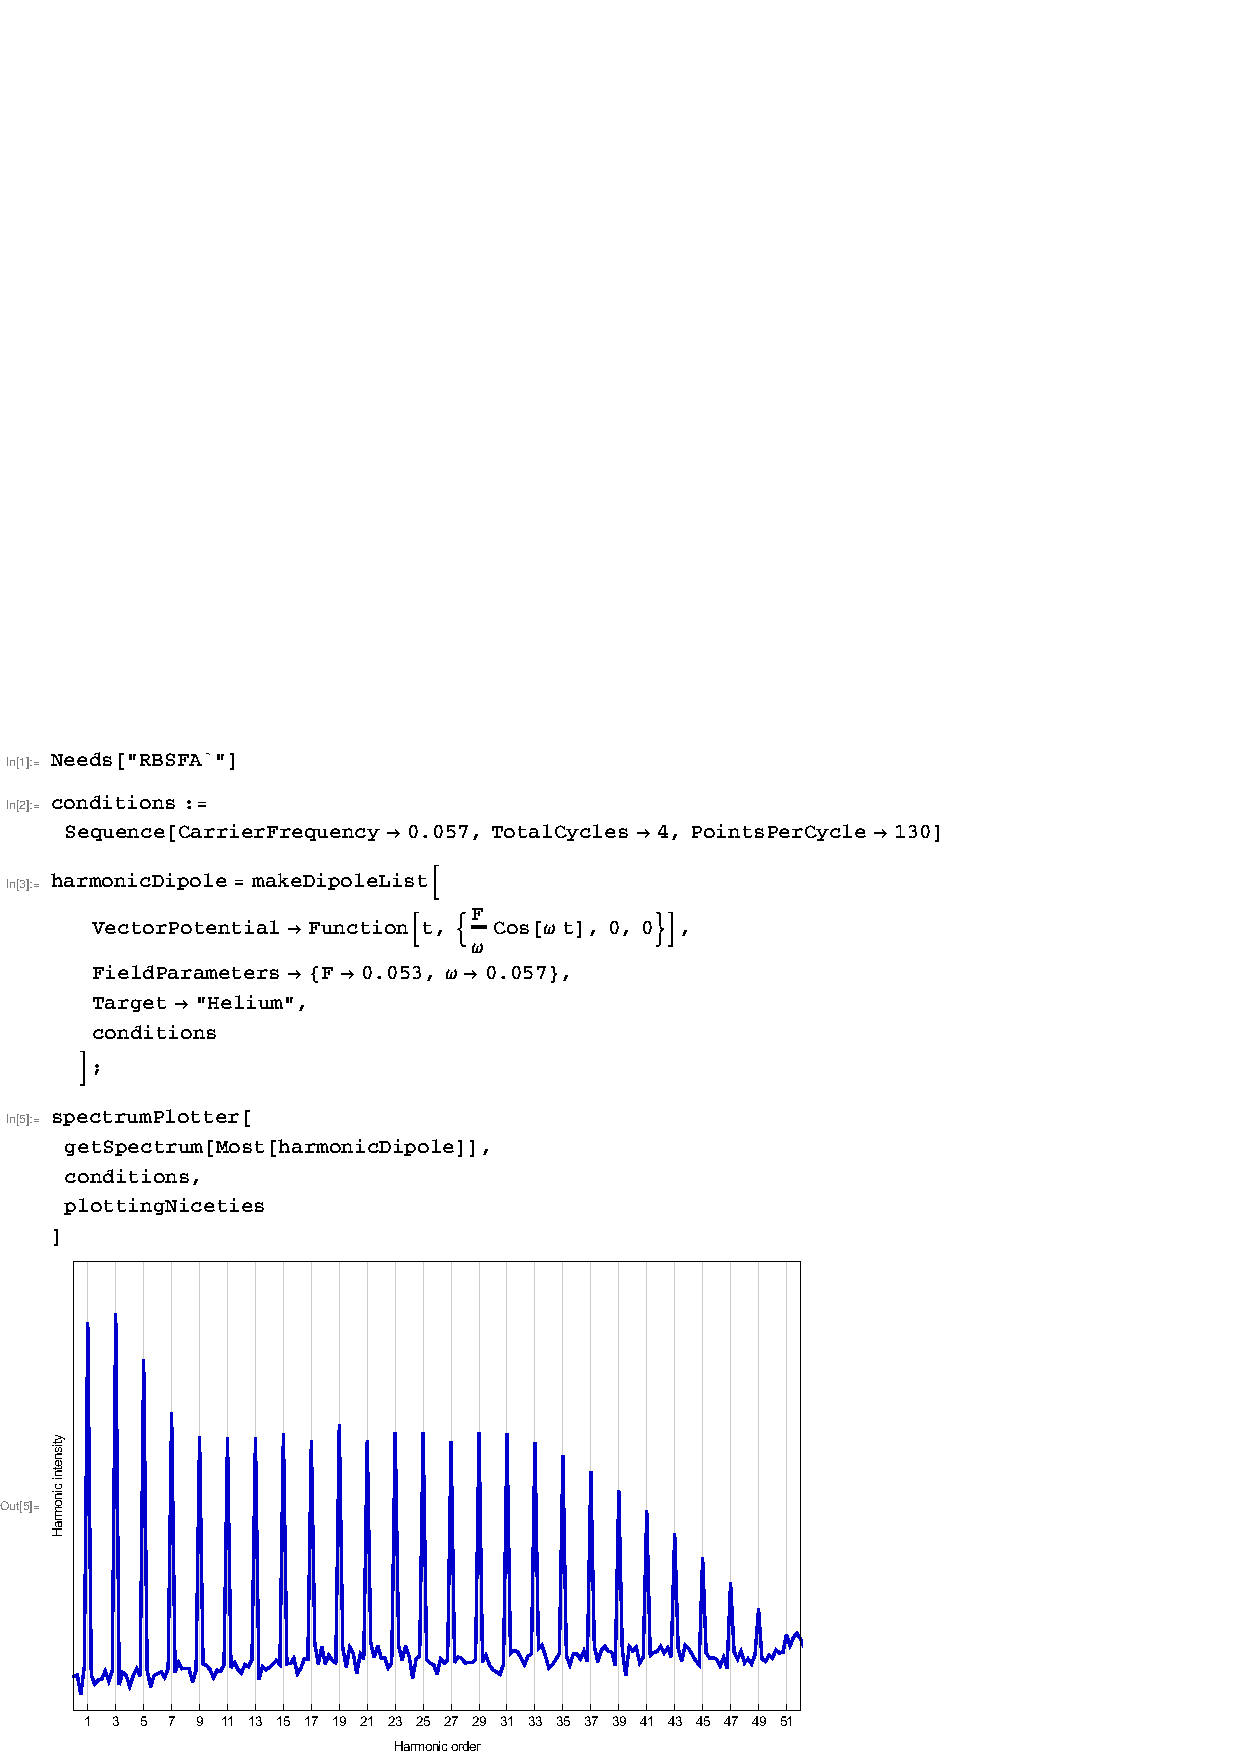
\includegraphics[width=0.9\textwidth]{7-HHG-intro/Figures/figure7C.pdf}
  }
  \captionsetup{width=0.96\textwidth}
  \caption[
  Sample screenshot of the RBSFA code used to calculate HHG spectra
  ]{
  Screenshot of the code used to produce \reffig{f7-standard-harmonic-spectrum} with the RB-SFA Mathematica package available as \citer{RB-SFA}. The code implements the standard SFA theory developed in this chapter, along with the beyond-dipole corrections discussed in chapter~\ref{chap:nondipole-HHG}, and it is simple and easy to use.
  }
\label{f7-RBSFA-screenshot}
\end{figure}


At this point, having reviewed the general features of high-order harmonic generation, and having built the SFA framework we will use for calculations, we now turn to its applications in the following two chapters.































